\chapter{Introduction}
\label{ch:introduction}
Inferix is a decentralized GPU network for visual computing and AI, it is built to bridge the needs of users and hardware owners. Its solution meets real-world problems across a range of industries, not only for the AI field but also for high-quality rendering needs. Users (e.g.~3D graphics artists, game developers, enterprises) who need GPU computing power for rendering high-quality graphics can use Inferix system to continuously access these precious resources with faster processing time and more efficient spending.
\begin{figure}[h]
    \centering
    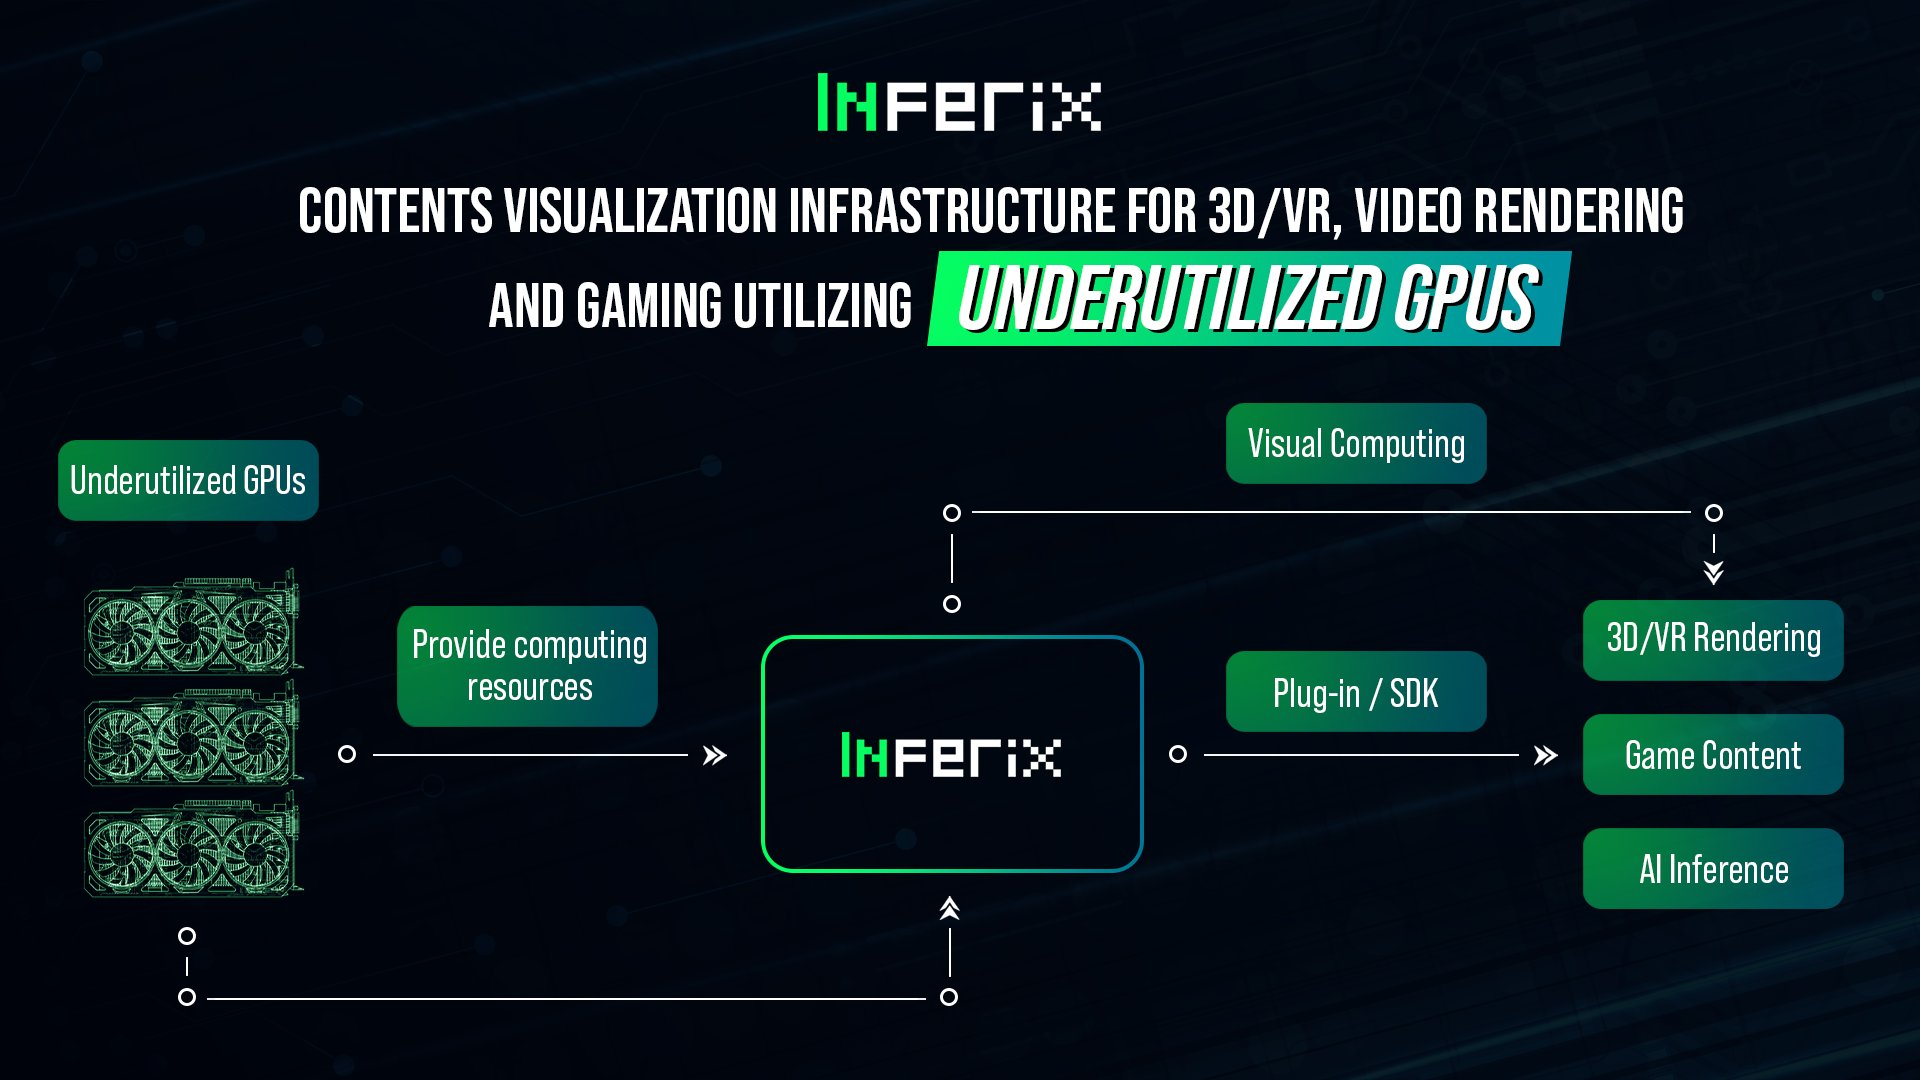
\includegraphics[width=0.8\textwidth]{inferix_high_level_architecture.jpg}
    \caption{High level architecture}
    \label{fig:inferix_rendering_network_high_level}
\end{figure}
Owners of GPUs can share idle resources to Inferix network and earn long-term passive income while simultaneously balancing their main jobs or leisure activities.

In this document, we focus mainly on the internal details of Inferix 3D graphics rendering network.


% Inferix provides a decentralized 3D graphics rendering service: remote people can submit Blender graphics scenes then receive rendered images and videos, others can join the service to let their computing resources for hire. Since the graphic rendering processes are intensively resources (GPU, RAM, disk storage, etc.) consuming and not everyone possessing these resources, Inferix regulates this exigence by in the one hand helping artists get their jobs done without equipping very high-end workstations. In the other hand, it allows individuals making profit from their unused high-performance computation resources.


\section[Rendering network]{Rendering network}
The graphics rendering service consists in a network of physically decentralized machines called \emph{nodes} which are of $3$ kinds: \emph{manager}, \emph{worker} and \emph{verifier}. The \emph{managers} and \emph{verifiers} are dedicated machines of Inferix while the \emph{workers} are machines joined of GPU owners. The number of \emph{workers} is normally much larger than the number of \emph{managers} and \emph{verifiers}.
\begin{figure}[h]
    \centering
    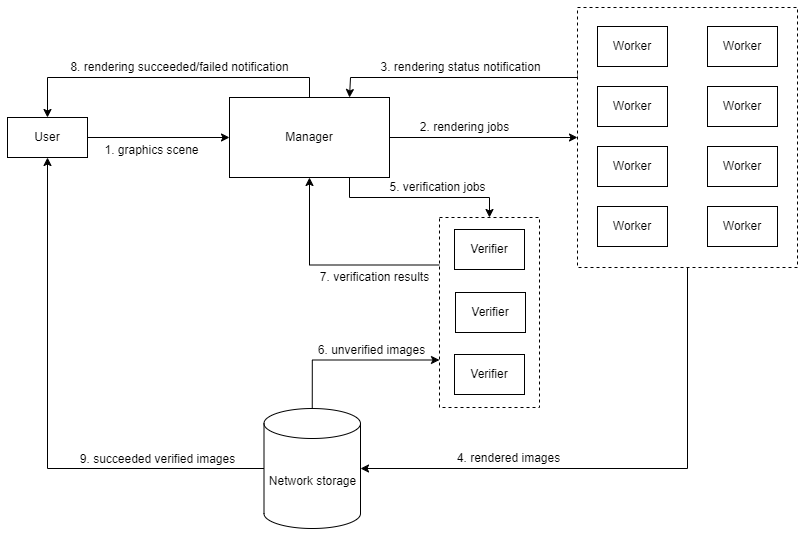
\includegraphics[width=0.8\textwidth]{rendering_service.png}
    \caption[Graphics rendering flow]{Graphics rendering flow}
    \label{fig:rendering_service}
\end{figure}
A typical rendering session is shown in~\autoref{fig:rendering_service}:
\begin{enumerate}
    \item A user submits a graphics scene to some \emph{manager} using the Inferix plugin for client.
    \item Receiving the graphics scene, the \emph{manager} builds corresponding rendering jobs consisting of several parameters (range of rendered images, format of the rendering ouput, \dots), then pushes these jobs into a rendering job queue. It maintains a pool of \emph{workers}, jobs from the job queue are dispatched to workers in the pool.
    % it dispatches jobs from the job queue to workers in the pool.
    \item Receiving a rendering job, a \emph{worker} renders the attached graphics scene using the parameters given by the job. When the rendering finishes, it sends the rendered images to a storage then notifies the \emph{manager}
    \item 
\end{enumerate}
 directly using the Inferix plugin for Blender (or via some Web interface!?). The \emph{manager} creates a job corresponding to this graphics scene, queues this job into a pool then dispatches to \emph{workers} which do the rendering. The rendered images will be sent back from \emph{workers} to several \emph{verifiers} which check if the images are valid. The validity is notified to the \emph{manager} to accept or reject the rendered results: a job is considered valid only if all results of this job pass the verification, in this case the results will be sent back to users.

(...add a figure here describing the high-level architect of rendering service)

\section[Output verification]{Output verification}\label{sec:output_verification}
In the network, \emph{workers} are mostly workstations (beside Inferix's dedicated servers) joined by users which want to make profit from their unused computing resources. There is no control (except initial hardware requirements to join the network!?) over these machines, so the graphics rendering is proceeded without being controlled. In order to guarantee that the graphics scenes are correctly rendered, we propose a mechanism called \emph{Active Noise Generation and Verification} which is presented in detail in~\autoref{ch:scene_watermarking}.

(...add a concrete example about an attack)